% =================================================================================
% TAP REPORT
% Author: Jack Davison
% A nice looking TAP report with a sensible structure. Not all sections will always
% be relevant (e.g., early on you probably won't have publications to talk about!)
% =================================================================================

\documentclass[12pt]{article}

% =================================
% PACKAGES ========================
% =================================

\usepackage[top=2.5cm, bottom=2.5cm, left=2.5cm, right=2.5cm, headheight = 15pt]{geometry}

% Set-up commands
\usepackage[T1]{fontenc}
\usepackage[utf8]{inputenc}
\usepackage{lmodern}
\usepackage[english]{babel}
\usepackage[autostyle]{csquotes}
\usepackage{blindtext}

% Better text
\usepackage{ragged2e} %text alignment
\usepackage{xcolor}   %colors
\usepackage{enumitem} %better control over lists
\usepackage{fancyhdr}

% Better Tables
\usepackage{tabularx} %alignments
\usepackage{booktabs} %toprule, midrule, etc.
\newcolumntype{L}{>{\RaggedRight}X} %new column (fixed width, left aligned)
\newcolumntype{R}{>{\RaggedLeft}X} %new column (fixed width, right aligned)

% Better Figures
\usepackage{graphicx} %figures
\usepackage{pdfpages} %insert whole pdf as a page

% Better Commands
\usepackage{xspace} %allow commands to detect punctuation
\usepackage[version=4]{mhchem} %chemistry

% Better Navigation
\usepackage{hyperref} %clickable links
\AtBeginDocument{\def\chapterautorefname{Chapter}} %Capitalise "chapter" in \autoref
\AtBeginDocument{\def\sectionautorefname{Section}} %Capitalise "section" in \autoref
\AtBeginDocument{\def\subsectionautorefname{Subsection}} %Capitalise "subsection" in \autoref

% Better Captions
\usepackage[font=small,labelfont=bf]{caption}

% Better Code
\usepackage{listings}           % For formatted code blocks

% Only for template
\usepackage{mwe}
\usepackage{lipsum}

% Set-up References
\usepackage[
  backend = biber, 
  natbib = true,
  style = numeric-comp,
  sorting = none,
  url = true,
  isbn = false,
  uniquename = false,
  maxcitenames = 1,
  maxbibnames = 99,
  date = year,
  giveninits = true
]{biblatex}

\DeclareNameAlias{author}{family-given}
\renewbibmacro{in:}{}

\addbibresource{bib/references.bib}
\addbibresource{bib/ref2.bib}

% Set-up Colours
\definecolor{mygray}{gray}{0.7}
\definecolor{airforceblue}{rgb}{0.36, 0.54, 0.66}

\hypersetup{
  colorlinks = true,
  urlcolor = airforceblue, 
  citecolor = airforceblue, 
  linkcolor = airforceblue
}

% Formatting of code blocks
\definecolor{green_comment}{rgb}{0,0.6,0}

\lstset{
  language = R,
  basicstyle = \footnotesize,
  commentstyle = \color{green_comment},
  frame = single,
  numbers = left
}

% =================================
% COMMANDS ========================
% =================================

% chemistry
\newcommand{\nox}{\ce{NO_{x}}\xspace}
\newcommand{\notwo}{\ce{NO2}\xspace} 
\newcommand{\cotwo}{\ce{CO2}\xspace}
\newcommand{\ammonia}{\ce{NH3}\xspace}

% units
\newcommand{\gkg}{g~kg\textsuperscript{-1}\xspace}
\newcommand{\gkm}{g~km\textsuperscript{-1}\xspace}


% =================================
% META ============================
% =================================

\newcommand{\thesistitle}{My amazing project title}

\title{
    \textbf{\thesistitle} \\~\\
    \large n\textsuperscript{th} Month TAP Report
    }
\author{My Name}

% =================================
% DOCUMENT ========================
% =================================

% title page & contents
\begin{document}
\maketitle
\begin{figure}[h!]%graphical abstract?
    \centering
    \includegraphics[width = .4\linewidth]{example-image-a}
\end{figure}
\tableofcontents
\bigskip
\noindent Also find attached the unpublished manuscript, \textit{``My cool paper''}.
\newpage

% start fancy headers
\pagestyle{fancy}
\rhead{\slshape\nouppercase{\leftmark}}
\lhead[E,O]{}

% overview section
\section{Overview}

\textbf{Here is where I provide background to my project, ``\thesistitle'' \dots} \lipsum[1]

\textbf{Here is where I talk about what I've achieved so far\dots} \lipsum[2]

\textbf{Here are some key achievements since the last TAP\dots} \lipsum[3]

This report presents a very brief summary of the work I have done and activities I have been a part of since the previous TAP meeting.

\textbf{Here is where I might mention what each section is about\dots}

% writing section (for third years mainly!)
\newpage \section{Writing}\label{sec:writing}

\subsection{Publications}\label{sec:pubs}

\autoref{tab:pubs} outlines my involvement in publications in my PhD thusfar.

\begin{table}[h]
    \centering
    \begin{tabularx}{\linewidth}{cXlc}
        \toprule
             & \textbf{Title} & \textbf{Journal}  & \textbf{Ref.} \\
        \midrule
            \multicolumn{4}{l}{\textbf{First Author Papers}} \\
        \midrule
            P & An incredible paper about all sorts of cool stuff & STOTEN & \cite{Davison2020} \\
            \\
            R & A super cool paper that's under review\dots & ES\&T & [--] \\
            \\
        \midrule
            \multicolumn{4}{l}{\textbf{Other Papers}} \\
        \midrule
             P & A nice paper that someone else took the lead on & ES\&T & \cite{Grange2020}\\~\\
             W & \textcolor{gray}{``Untitled Paper we're writing at the moment''} & ES\&T & [--] \\~\\
        \bottomrule
    \end{tabularx}
    \caption{My involvement in publications so far in my PhD. The first column shows whether the paper has been \textbf{P}ublished, is Under \textbf{R}eview, or is being \textbf{W}ritten.}
    \label{tab:pubs}
\end{table}

\textbf{Here is where I might talk a bit about these papers - are they going to be chapters? Will all my chapters be papers?} \lipsum[1]

\clearpage\subsection{Thesis Outline \& Plan}\label{sec:thesis}

Listed below is a general thesis outline. Any chapter titles in quotation marks are placeholders. An asterisk (\textasteriskcentered) indicates that the chapter has already been written and/or published.

\begin{table}[h]
    \centering
    \begin{tabularx}{\linewidth}{llX}
        & 1 & \textbf{Introduction:} A very brief opening chapter setting the scene and covering the overall aims of the thesis. \\~\\
        
        & 2 & \textbf{Literature Review:} A review of all the relevant literature. \\~\\
        
        \textasteriskcentered & 3 & \textbf{My first science chapter\dots:} A paper I've already written. \\~\\
        
        & 4 & \textbf{My second science chapter\dots:} A paper I've not written yet but will! \\~\\
        
        \textasteriskcentered & 5 & \textbf{My third science chapter\dots:} Another paper. \\~\\
        
        & 6 & \textbf{Conclusion}. An attempt to tie everything together; further discuss the implications of the presented work; suggest future directions.
    \end{tabularx}
\end{table}

\textbf{Here is where I might talk a bit about my thesis plan, and how it is going} \lipsum[2]

\newpage

% Research section - to talk about PhD project
\section{Research}\label{sec:research}

\subsection{Research Theme 1}\label{sec:rt1}
\subsection{Research Theme 2}\label{sec:rt2}
\subsection{Research Theme 3}\label{sec:rt3}

\textbf{I might start talking about different bits of research I've done now.} \lipsum[5]

\textbf{Maybe I'll put in a figure and/or a table.}

\begin{table}[bht]
    \centering
    \begin{tabularx}{\linewidth}{lXXXX}
        \toprule
        \textbf{Species} & \textbf{Petal Length} & \textbf{Petal Width} & \textbf{Sepal Length} & \textbf{Sepal Width} \\ 
        \midrule
        Setosa & 1.462 & 0.246 & 5.006 & 3.428 \\ 
        Versicolor & 4.260 & 1.326 & 5.936 & 2.770 \\ 
        Virginica & 5.552 & 2.026 & 6.588 & 2.974 \\ 
        \bottomrule
    \end{tabularx}
    \caption{Mean values from Fischer's ``iris'' data set.}
    \label{tab:wide_tab}
\end{table}

\begin{figure}[bht]
    \centering
    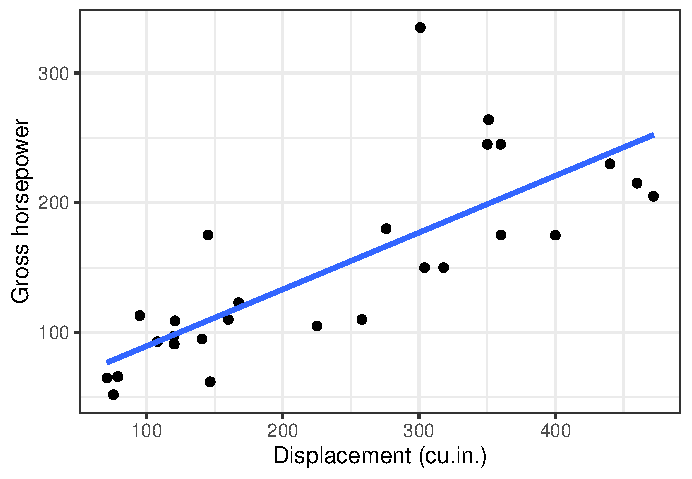
\includegraphics[width=.7\linewidth]{figures/myplot.pdf}
    \caption{A lovely R plot, saved as a PDF rather than a PNG or JPEG.}
    \label{fig:mtcars}
\end{figure}

% "Other Activities" - because there's more to being a PhD Student than research
\newpage\section{Other Activities}\label{sec:other}

This brief section outlines other achievements and activities I have taken part in over the last 6 months.

\begin{itemize}
    \item \textbf{Teaching:} I've been teaching\dots
    \item \textbf{Learning:} I went on this course\dots
    \item \textbf{Outreach:} I did\dots
    \item \textbf{Prize:} I won\dots.
\end{itemize}

% References
\newpage\section{References}
{\RaggedRight\sloppy
\printbibliography[heading = none]}
\end{document}